\documentclass[b5paper]{ujreport}
\usepackage{bxpapersize}
\usepackage[dvipdfmx]{graphicx}
\usepackage{geometry}

\geometry{left=25mm,right=25mm,top=30mm,bottom=30mm}

\begin{document}

\begin{titlepage}
\begin{center}
\vspace*{3pt}
{\large\itshape SKSAT vol.1}
\vspace{12pt} \\
\begin{tabular}{rl}
著 sksat
\end{tabular}
\vspace{3pt} \\
\today \vspace{12pt} \\
\end{center}
\end{titlepage}

\chapter*{序}
部誌の原稿.今のところは物理数学の初歩と,数値計算の理論・実装について.

後輩用のテキストとしての役目もあり.

\chapter{物理数学入門}
\section{運動の3法則}
\subsection{力のつり合いと作用反作用の法則}

まずは,静止している物体について考えてみよう.

\begin{figure}[htbp]
\begin{center}
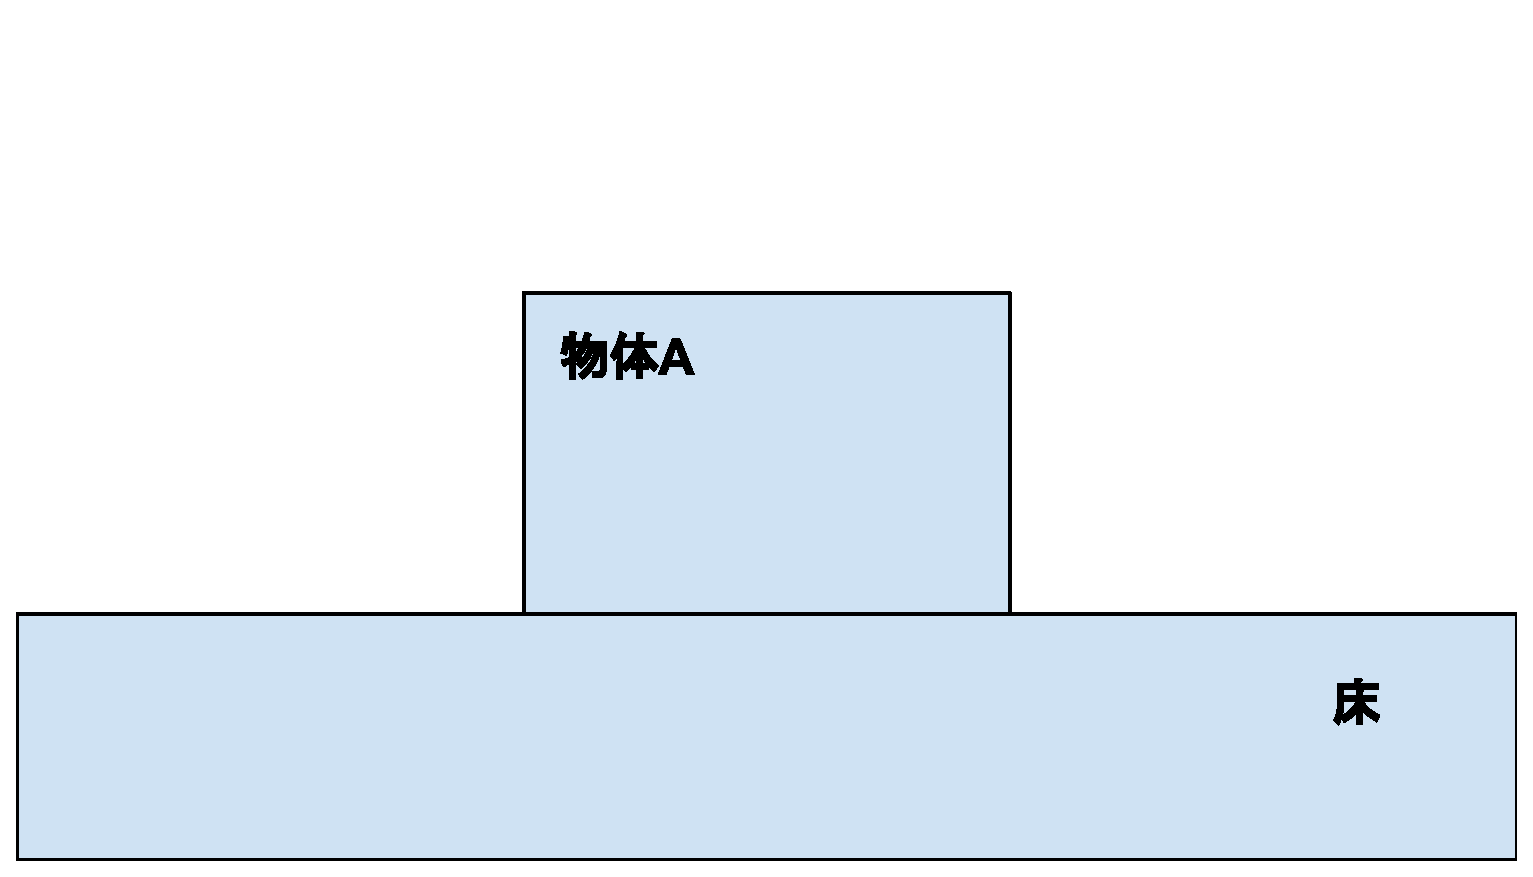
\includegraphics[width=4cm]{img/床の上で静止している物体.eps}
\end{center}
\caption{床の上で静止している物体}
\label{object_on_floor}
\end{figure}

図\ref{object_on_floor}のように,床の上に静止している物体Aがあるとする.
このとき,物体Aにはいったいどのような力が働いているだろうか?
まず最初に思い浮かぶのは,図\ref{object_on_floor_with_gravity}の矢印のような重力である.

\begin{figure}[htbp]
\begin{center}
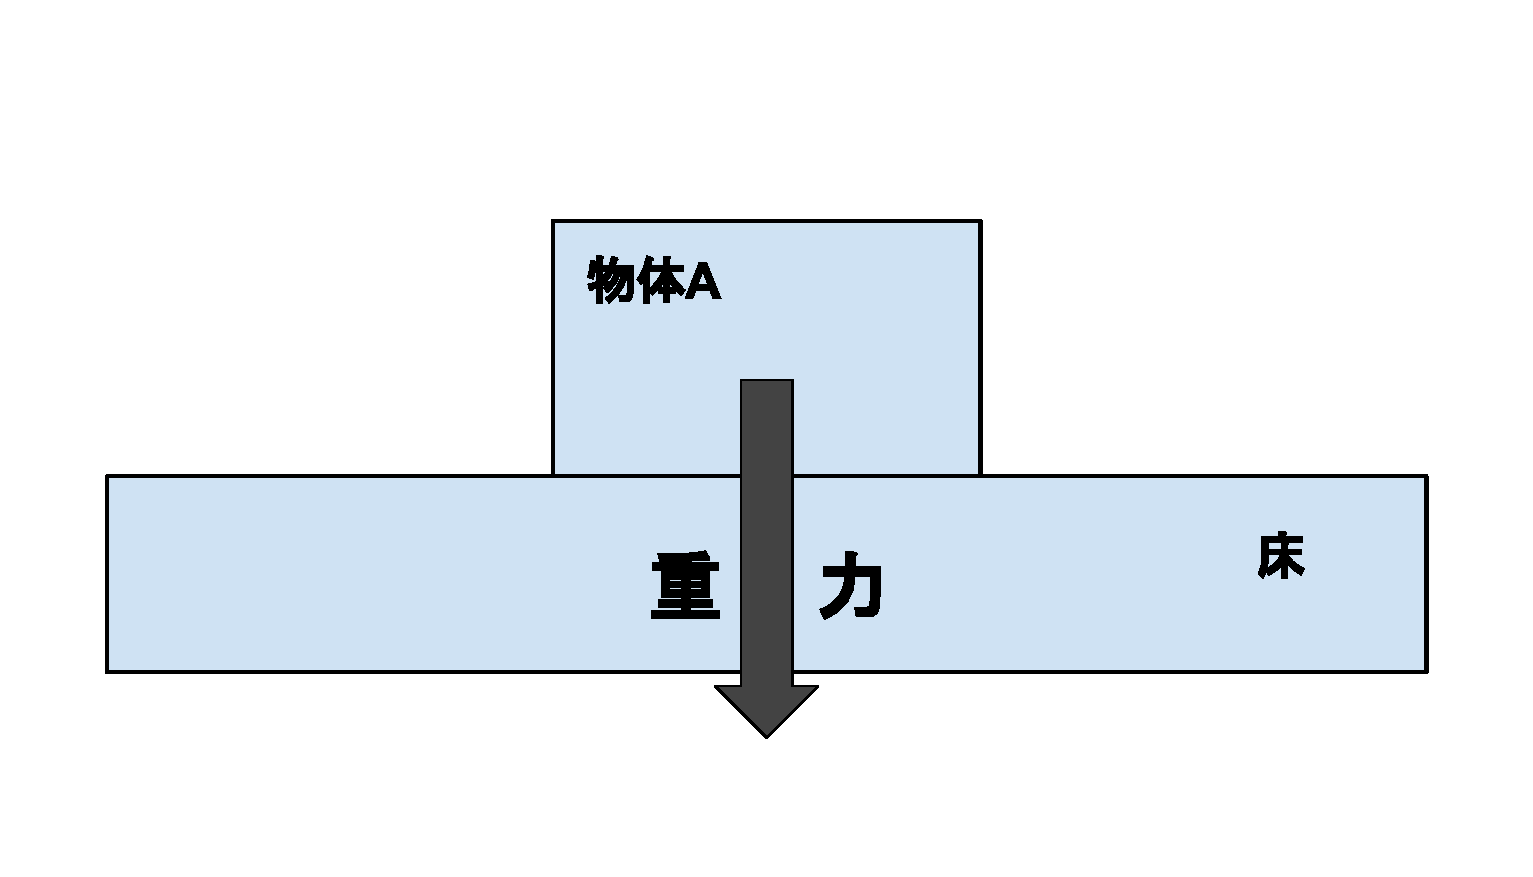
\includegraphics[width=5cm]{img/力のつり合い-重力.eps}
\end{center}
\caption{物体Aに働く重力}
\label{object_on_floor_with_gravity}
\end{figure}

しかし,物体Aに働いている力が重力だけだと,物体A重力によって鉛直下向き
\footnote{鉛直とは,重りを糸で吊り下げた時の糸が示す方向.つまり,重力が働く方向のこと.鉛直下向きの対義語は「鉛直上向き」.}
に引っ張られ,床にめり込んでいってしまう.

\begin{figure}[htbp]
\begin{center}
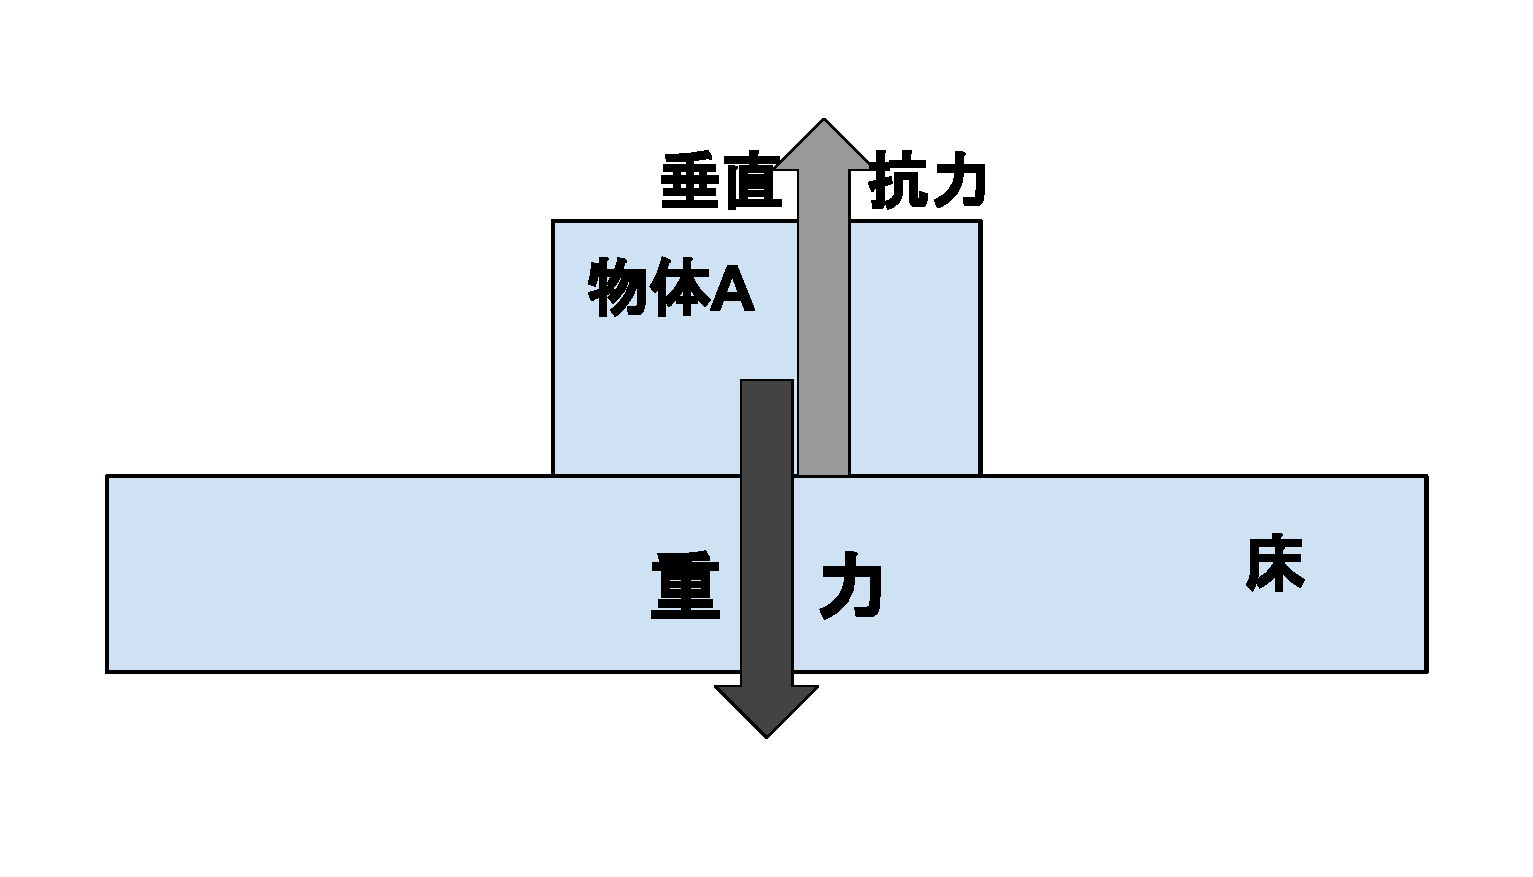
\includegraphics[width=6cm]{img/力のつり合い.eps}
\end{center}
\label{object_on_floor_with_balance}
\caption{力のつり合い}
\end{figure}

このことから,物体Aに働く力は重力だけではなく,図\ref{object_on_floor_with_balance}のように,
床からも力を受けている,ということが分かる.
物体Aの運動を妨げるように,物体Aが床から受けているような力のことを抗力という.
特に,物体の面が他の物体に対して面と垂直な方向に及ぼす抗力のことを「垂直抗力」という\footnote{『物理基礎』における定義}.

この場合においては物体Aが静止しているため,垂直抗力の大きさは物体Aが受ける重力の大きさに等しく,また,その向きは鉛直上向きである.

このように,物体に複数の力が同時に働いていても,それらを合わせて考えると,
力が全く働いていないのと同等とみなせるとき,これらの\bfseries{力はつりあっている}という.

\chapter{数値計算の理論}
\section{はじめに}
現在僕は,ロケットの軌道や,N体問題
\footnote{後述するが,簡単に言うと,「相互作用する3体以上の質点系」のこと.本稿においては複数の天体の運動を考える問題と思ってくれて構わない.}
のコンピュータ・シミュレーションを行っている.

\section{シミュレーションとは}
シミュレーションとはそもそも,何らかのシステムが従っている法則を抽出、モデル化し、模擬することである.
その「模擬」する方法は特に決まっているわけではなく,紙とペンかもしれないし,小さな模型\footnote{風洞実験などがこれに当てはまる.}かもしれないし,コンピュータプログラムかもしれない.


\begin{thebibliography}{99}
\bibitem{物理基礎} 國友正和ほか10名 『物理基礎』 (数研出版,平成28年発行)
\end{thebibliography}

\end{document}
